\documentclass{article}
\usepackage{tikz}
\begin{document}
% 1.坐标系统
% tikz的xy(或xyz)坐标系统,是坐标内的x/y值(x/y/z值)相对于单位值的移动
% 修改x/y值的单位值
%   1)x={<dimension> | <coordinate>}
%     dimension即沿x轴移动指定距离
%     coordinate即沿x/y轴分别移动指定距离
%   2)y={<dimension> | <coordinate>}
%     dimension即沿y轴移动指定距离
%     coordinate即沿x/y轴分别移动指定距离
\begin{tikzpicture}
    \draw[->] (-3,0) -- (3,0) node[below]{$x$};
    \draw[->] (0,-3) -- (0,3) node[left]{$y$};
    \draw[x=2cm] (0,0) -- (1,1);
    \draw[x={(1cm,2cm)},red] (0,0) -- (-1,0);
\end{tikzpicture}



% 2.坐标转换
% tikz的转化系统,本质是直接对坐标进行转化
%   1)偏移(shift)
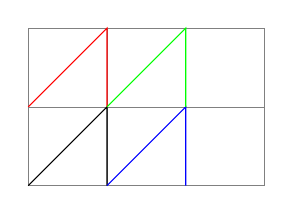
\begin{tikzpicture}
    % shift={<coordinate>}
    %   坐标在x/y轴上的偏移
    % xshift=<dimension>
    %   在x轴上的偏移
    % yshift=<dimension>
    %   在y轴上的偏移
    \draw[help lines] (0,0) grid (3,2);
    \draw (0,0) -- (1,1) -- (1,0);
    \draw[xshift=1cm,blue] (0,0) -- (1,1) -- (1,0);
    \draw[yshift=1cm,red] (0,0) -- (1,1) -- (1,0);
    \draw[shift={(1cm,1cm)},green] (0,0) -- (1,1) -- (1,0);
\end{tikzpicture}
\vspace{2cm}

%   2)伸缩(scale)
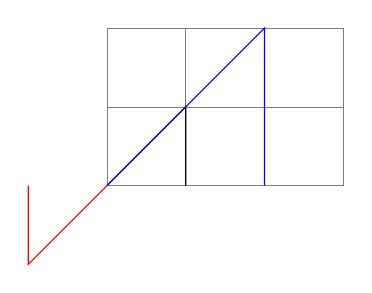
\begin{tikzpicture}
    % scale=<factor>
    %   根据坐标到原点的距离进行伸缩
    % scale around={<factor>:<coordinate>}
    %   根据坐标到指定点的距离进行伸缩
    % xscale=<factor>
    %   根据坐标到原点的距离,只在x轴上进行伸缩
    % yscale=<factor>
    %   根据坐标到原点的距离,只在y轴上进行伸缩
    \draw[help lines] (0,0) grid (3,2);
    \draw (0,0) -- (1,1) -- (1,0);
    \draw[scale=2,blue] (0,0) -- (1,1) -- (1,0);
    \draw[scale=-1,red] (0,0) -- (1,1) -- (1,0);
\end{tikzpicture}\vspace{2cm}

%   3)旋转(rotate)
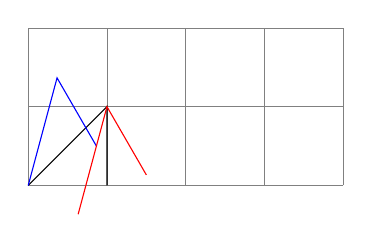
\begin{tikzpicture}
    % rotate=<degree>
    %   坐标沿原点旋转
    % rotate around={<degree>:<coordinate>}
    %   坐标沿指定点旋转
    % rotate around x=<angle>
    %   绕x轴旋转指定度数
    % rotate around y=<angle>
    %   绕y轴旋转指定度数
    % rotate around z=<angle>
    %   绕z轴旋转指定度数
    \draw[help lines] (0,0) grid (4,2);
    \draw (0,0) -- (1,1) -- (1,0);
    \draw[rotate=30,blue] (0,0) -- (1,1) -- (1,0);
    \draw[rotate around={30:(1,1)},red] (0,0) -- (1,1) -- (1,0);
\end{tikzpicture}
\vspace{2cm}

%   4)倾斜(slant)
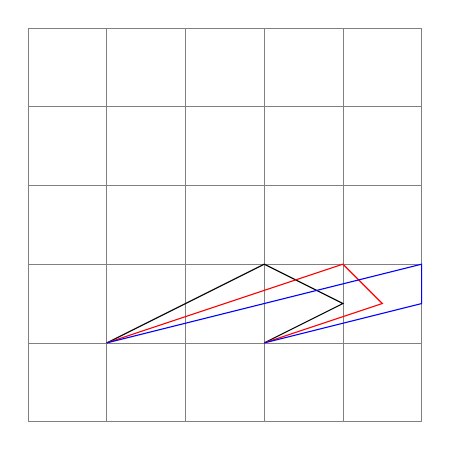
\begin{tikzpicture}
    % xslant=<factor>
    %   在x轴方向增加factor * y的值,结果为(x + factor * y, y),x轴上的值保持不变
    \draw[help lines] (-1,-1) grid (4,4);
    \draw (0,0) -- (2,1) -- (3,0.5) -- (2,0);
    \draw[xslant=1,red] (0,0) -- (2,1) -- (3,0.5) -- (2,0);
    \draw[xslant=2,blue] (0,0) -- (2,1) -- (3,0.5) -- (2,0);
\end{tikzpicture}

    % yslant=<factor>
    %   在y轴方向增加factor * x的值,结果为(x, y + factor * x),y轴上的值保持不变
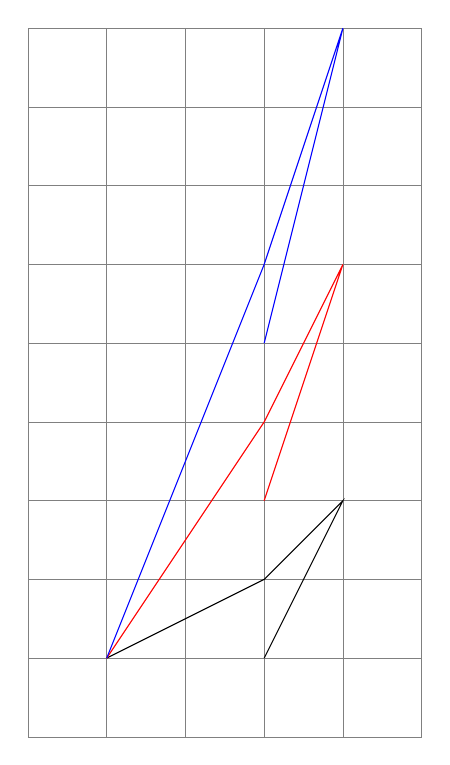
\begin{tikzpicture}
    \draw[help lines] (-1,-1) grid (4,8);
    \draw (0,0) -- (2,1) -- (3,2) -- (2,0);
    \draw[yslant=1,red] (0,0) -- (2,1) -- (3,2) -- (2,0);
    \draw[yslant=2,blue] (0,0) -- (2,1) -- (3,2) -- (2,0);
\end{tikzpicture}\vspace{2cm}

%   5)矩阵变化
%     cm={<a>,<b>,<c>,<d>,<coordinate>}
%       (ax+cy,bx+dy)+(coordinate)的结果

%   6)变化叠加
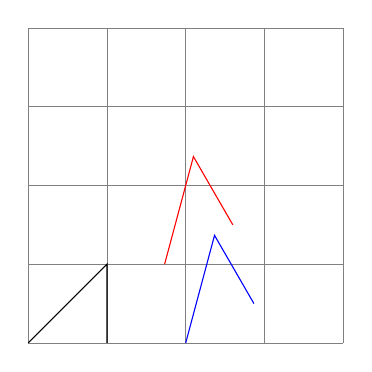
\begin{tikzpicture}
    \draw[help lines] (0,0) grid (4,4);
    \draw (0,0) -- (1,1) -- (1,0);
    % 先沿x轴右移2cm,在旋转30度
    \draw[rotate=30,xshift=2cm,red] (0,0) -- (1,1) -- (1,0);
    % 先旋转30度,再沿x轴右移2cm
    \draw[xshift=2cm,rotate=30,blue] (0,0) -- (1,1) -- (1,0);
\end{tikzpicture}

%   7)坐标系统转换
%     直接将坐标系统进行转换,scale时,影响线条宽度等
%     transform canvas={<options>}
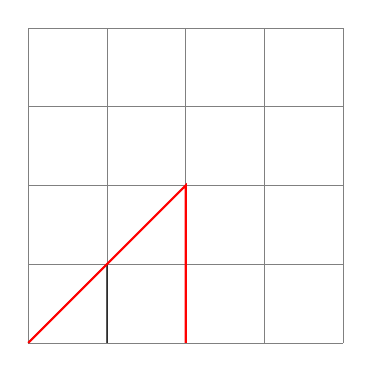
\begin{tikzpicture}
    \draw[help lines] (0,0) grid (4,4);
    \draw (0,0) -- (1,1) -- (1,0);
    \draw[transform canvas={scale=2},red] (0,0) -- (1,1) -- (1,0);
\end{tikzpicture}

\end{document}
